%!TeX encoding = UTF-8
%!TeX program = xelatex
\documentclass[notheorems, aspectratio=54]{beamer}
% aspectratio: 1610, 149, 54, 43(default), 32

\usepackage{latexsym}
\usepackage{amsmath,amssymb}
\usepackage{mathtools}
\usepackage{color,xcolor}
\usepackage{graphicx}
\usepackage{algorithm}
\usepackage{amsthm}
\usepackage{lmodern} % 解决 font warning
% \usepackage[UTF8]{ctex}
\usepackage{animate} % insert gif

\usepackage{lipsum} % To generate test text 
\usepackage{ulem} % 下划线,波浪线

\usepackage{listings} % display code on slides; don't forget [fragile] option after \begin{frame}
\usepackage{verbatim}
\makeatletter
\def\verbatim@font{\tiny\ttfamily}
\makeatother

% ----------------------------------------------
% tikx
\usepackage{framed}
\usepackage{tikz}
\usepackage{pgf}
\usetikzlibrary{calc,trees,positioning,arrows,chains,shapes.geometric,%
    decorations.pathreplacing,decorations.pathmorphing,shapes,%
    matrix,shapes.symbols}
\pgfmathsetseed{1} % To have predictable results
% Define a background layer, in which the parchment shape is drawn
\pgfdeclarelayer{background}
\pgfsetlayers{background,main}

\definecolor{AmethystPurple}{HTML}{AEAEDF}
% define styles for the normal border and the torn border
\tikzset{
  normal border/.style={AmethystPurple, decorate, 
     decoration={random steps, segment length=2.5cm, amplitude=.7mm}},
  torn border/.style={AmethystPurple, decorate, 
     decoration={random steps, segment length=.5cm, amplitude=1.7mm}}}

% Macro to draw the shape behind the text, when it fits completly in the
% page
\def\parchmentframe#1{
\tikz{
  \node[inner sep=1.5em] (A) {#1};  % Draw the text of the node
  \begin{pgfonlayer}{background}  % Draw the shape behind
  \fill[normal border] 
        (A.south east) -- (A.south west) -- 
        (A.north west) -- (A.north east) -- cycle;
  \end{pgfonlayer}}}

% Macro to draw the shape, when the text will continue in next page
\def\parchmentframetop#1{
\tikz{
  \node[inner sep=2em] (A) {#1};    % Draw the text of the node
  \begin{pgfonlayer}{background}    
  \fill[normal border]              % Draw the ``complete shape'' behind
        (A.south east) -- (A.south west) -- 
        (A.north west) -- (A.north east) -- cycle;
  \fill[torn border]                % Add the torn lower border
        ($(A.south east)-(0,.2)$) -- ($(A.south west)-(0,.2)$) -- 
        ($(A.south west)+(0,.2)$) -- ($(A.south east)+(0,.2)$) -- cycle;
  \end{pgfonlayer}}}

% Macro to draw the shape, when the text continues from previous page
\def\parchmentframebottom#1{
\tikz{
  \node[inner sep=2em] (A) {#1};   % Draw the text of the node
  \begin{pgfonlayer}{background}   
  \fill[normal border]             % Draw the ``complete shape'' behind
        (A.south east) -- (A.south west) -- 
        (A.north west) -- (A.north east) -- cycle;
  \fill[torn border]               % Add the torn upper border
        ($(A.north east)-(0,.2)$) -- ($(A.north west)-(0,.2)$) -- 
        ($(A.north west)+(0,.2)$) -- ($(A.north east)+(0,.2)$) -- cycle;
  \end{pgfonlayer}}}

% Macro to draw the shape, when both the text continues from previous page
% and it will continue in next page
\def\parchmentframemiddle#1{
\tikz{
  \node[inner sep=2em] (A) {#1};   % Draw the text of the node
  \begin{pgfonlayer}{background}   
  \fill[normal border]             % Draw the ``complete shape'' behind
        (A.south east) -- (A.south west) -- 
        (A.north west) -- (A.north east) -- cycle;
  \fill[torn border]               % Add the torn lower border
        ($(A.south east)-(0,.2)$) -- ($(A.south west)-(0,.2)$) -- 
        ($(A.south west)+(0,.2)$) -- ($(A.south east)+(0,.2)$) -- cycle;
  \fill[torn border]               % Add the torn upper border
        ($(A.north east)-(0,.2)$) -- ($(A.north west)-(0,.2)$) -- 
        ($(A.north west)+(0,.2)$) -- ($(A.north east)+(0,.2)$) -- cycle;
  \end{pgfonlayer}}}

% Define the environment which puts the frame
% In this case, the environment also accepts an argument with an optional
% title (which defaults to ``Example'', which is typeset in a box overlaid
% on the top border
\newenvironment{parchment}[1][Example]{%
  \def\FrameCommand{\parchmentframe}%
  \def\FirstFrameCommand{\parchmentframetop}%
  \def\LastFrameCommand{\parchmentframebottom}%
  \def\MidFrameCommand{\parchmentframemiddle}%
  \vskip\baselineskip
  \MakeFramed {\FrameRestore}
  \noindent\tikz\node[inner sep=1ex, draw=black!20,fill=AmethystPurple, 
          anchor=west, overlay] at (0em, 1em) {\sffamily#1};\par}%
{\endMakeFramed}

% ----------------------------------------------

\mode<presentation>{
    \usetheme{Berkeley}
    % Boadilla CambridgeUS
    % default Antibes Berlin Copenhagen
    % Madrid Montpelier Ilmenau Malmoe
    % Berkeley Singapore Warsaw
    \usecolortheme{dolphin}
    % beetle, beaver, orchid, whale, dolphin
    \useoutertheme{infolines}
    % infolines miniframes shadow sidebar smoothbars smoothtree split tree
    \useinnertheme{circles}
    % circles, rectanges, rounded, inmargin
}
% 设置 block 颜色
\setbeamercolor{block title}{bg=AmethystPurple,fg=white}

\newcommand{\reditem}[1]{\setbeamercolor{item}{fg=red}\item #1}

% 缩放公式大小
\newcommand*{\Scale}[2][4]{\scalebox{#1}{\ensuremath{#2}}}

% 解决 font warning
\renewcommand\textbullet{\ensuremath{\bullet}}

% verbatim


% ---------------------------------------------------------------------
% flow chart
\tikzset{
    >=stealth',
    punktchain/.style={
        rectangle, 
        rounded corners, 
        % fill=black!10,
        draw=white, very thick,
        text width=6em,
        minimum height=2em, 
        text centered, 
        on chain
    },
    largepunktchain/.style={
        rectangle,
        rounded corners,
        draw=white, very thick,
        text width=10em,
        minimum height=2em,
        on chain
    },
    line/.style={draw, thick, <-},
    element/.style={
        tape,
        top color=white,
        bottom color=blue!50!black!60!,
        minimum width=6em,
        draw=blue!40!black!90, very thick,
        text width=6em, 
        minimum height=2em, 
        text centered, 
        on chain
    },
    every join/.style={->, thick,shorten >=1pt},
    decoration={brace},
    tuborg/.style={decorate},
    tubnode/.style={midway, right=2pt},
    font={\fontsize{10pt}{12}\selectfont},
}
% ---------------------------------------------------------------------

% code setting
\lstset{
    language=C++,
    basicstyle=\ttfamily\footnotesize,
    keywordstyle=\color{red},
    breaklines=true,
    xleftmargin=2em,
    numbers=left,
    numberstyle=\color[RGB]{222,155,81},
    frame=leftline,
    tabsize=4,
    breakatwhitespace=false,
    showspaces=false,               
    showstringspaces=false,
    showtabs=false,
    morekeywords={Str, Num, List},
}

% ---------------------------------------------------------------------

%% preamble
\title[Big Data Analysis In ACCRE]{Big Data Analysis In ACCRE}
\subtitle{Report on Learning Big Data Analysis: I}
\author{Fenglai Liu}
\institute[ACCRE]{fenglai@accre.vanderbilt.edu}

% -------------------------------------------------------------

\begin{document}

%% title frame
\begin{frame}
    \titlepage
\end{frame}

\section{Introduction}
\subsection{General Thoughts about My Future Role}
\begin{frame}
%    \frametitle{}

\begin{block}{What can I do as an application developer in ACCRE for big data analysis?}
\begin{itemize}
 \item Teaching;
 \item Programming/help people solving programming problems on big data;
 \item Helping people on using the cluster for big data analysis
\end{itemize}
\end{block}

 As a software developer the following points on the big data analysis interest me:
\begin{itemize}
 \item How to understand big data analysis from a traditional HPC programming view?
 \item How to use the big data analysis for practical projects?
\end{itemize}

\end{frame}

% -------------------------------------------------------------

\begin{frame}
%    \frametitle{}

For the second question, it can be divided into more specific questions:

\begin{description}
 \item [Data]
 \begin{itemize}
  \item what kind of level of data is ``big data'' and can be benefit from big data analysis?
  \item does big data analysis can be applied for all formats of data?
  \item the practical usage for big data analysis?
 \end{itemize}
  \item [Tools]
 \begin{itemize}
  \item comparisons between the big data languages and traditional languages, like scala VS C++?
  \item comparisons between the Spark VS openMP, MPI?  
 \end{itemize}
  \item [project]
 \begin{itemize}
  \item how large for a typical big data project?
  \item fast development?
  \item scalability on the cluster?
 \end{itemize}
\end{description} 

\end{frame}

% -------------------------------------------------------------

\begin{frame}
%    \frametitle{}

Upon Will's suggestion, I started the big data analysis journey by beginning from Spark and Scala/Python.
So in the following slices I will concentrate on the learning of Spark/Scala for the big data analysis.

Aspects to be covered in this talk and following talks: 
\begin{itemize}
 \item How can we understand Spark/Scala conceptually? Features comparing with C++/OpenMP/MPI etc.?
 \item How to use them for practical projects? From local jobs, to jobs on the cluster.
\end{itemize}


\end{frame}

% -------------------------------------------------------------

%% normal frame
\subsection{General View for Spark}
\begin{frame}
%    \frametitle{}

Spark is a ``framework'' for big data analysis. Why it is called a ``FRAMEWORK''? Because it is more than a collection of library:
\begin{description}
 \item [library] Spark can be used a a library for Scala/Python/Java programming languages.
 \item [REPL] Refers to Read-Evaluate-Print-Loop. Spark itself has an inner shell environment, 
 where the user can run the spark API in Scala interactively (key feature for fast development). 
 PySpark also has REPL function based on Python. 
\end{description}

\end{frame}

\begin{frame}
%    \frametitle{An Example}

    \begin{block}{How to think about the library VS. REPL for Spark?}
    REPL is a good feature for fast development and testing/debugging purpose(for example, C++/Java do not have it). It is also 
    good for teaching purpose, too. However, as the code growing and the project becomes more practical, library will be the only 
    choice for production implementation.     
    \end{block}
    
    In conclusion
   \begin{enumerate}
    \item  REPL $\Longrightarrow$ project;
    \item  implementation on local multi-threading env $\Longrightarrow$ practical project on cluster
   \end{enumerate}
      
\end{frame}

\section{Spark Components}
\subsection{SparkContext}
\begin{frame}[fragile]
    %\frametitle{An Example}

   \begin{block}{SparkContext: the main entry point for the Spark functionality.}
   The analog for the SparkContext  is like the MPI\_init function, which initializes the environment for cluster usage. 
   For MPI the configuration information is passed through the MPIEXEC etc. Here SparkContext can use SparkConf
   to set up the configuration information and initializes the Spark.
   \end{block}
   
   Scala example:
   \begin{verbatim}
    import org.apache.spark.SparkConf
    import org.apache.spark.SparkContext

    // define the spark conf
    val conf = new SparkConf()
    conf.setMaster("local[*]")  // using all of available cores 
    conf.setAppName("Spark App test") // set the application name

    // now let's create a new SparkContext according to conf
    val sc = new SparkContext(conf)
   \end{verbatim}     
  
\end{frame}

\subsection{RDD - Resilient Distributed Dataset}
\subsubsection{RDD Concept and Features}
\begin{frame}
 %   \frametitle{How can we improve the diagnosis}

RDD is simply a collection of data records. A similar thing to RDD is the block in HDFS. Conceptually 
RDD has following features:
\begin{itemize}
 \item in memory;
 \item resilient (fault-tolerant);
 \item partitioned and distributed;
 \item Lazy evaluated;
\end{itemize} 
  
\end{frame}


\begin{frame}
%    \frametitle{How can we improve the diagnosis}

\begin{block}{\textbf{in memory}}
 The biggest difference in my opinion between RDD and the block in HDFS is that RDD is stored in ``MEMORY''. It's able to transform
 different dataset like HDFS, Amazon S3, Cassandra etc. (disk-stored) into RDD for Spark use. Secondly, ``in-memory'' also enable the REPL possible. Data processing and data analysis can be performed interactively. 
\end{block}

\begin{figure}
 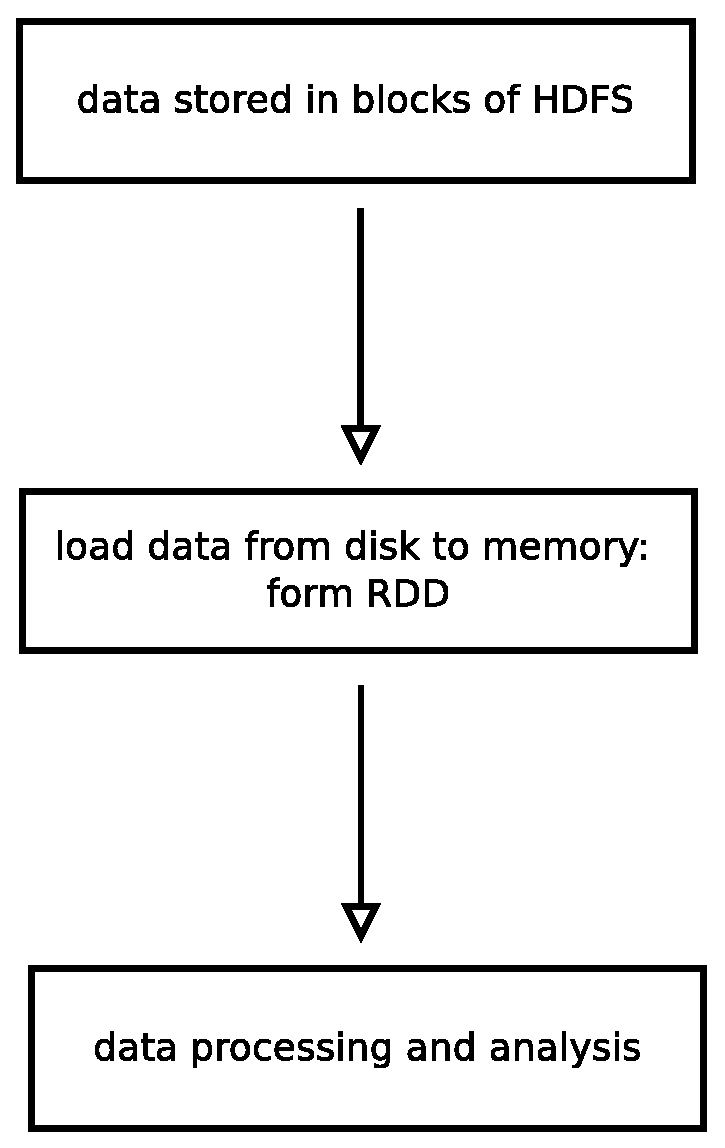
\includegraphics[scale=0.2]{rdd1}
\caption{simple flowchart for RDD}
\end{figure} 

 
\end{frame}


\begin{frame}
 %   \frametitle{How can we improve the diagnosis}

 

\end{frame}


\begin{frame}
  %  \frametitle{How can we improve the diagnosis}

  
\end{frame}

\begin{frame}
  %  \frametitle{How can we improve the diagnosis}

  
\end{frame}


\end{document}


